\documentclass[border=4mm]{standalone}
\usepackage[utf8]{inputenc}
\usepackage[T5]{fontenc}
\usepackage{mathptmx}
\usepackage{tikz}
\usetikzlibrary{arrows.meta,calc}

\begin{document}
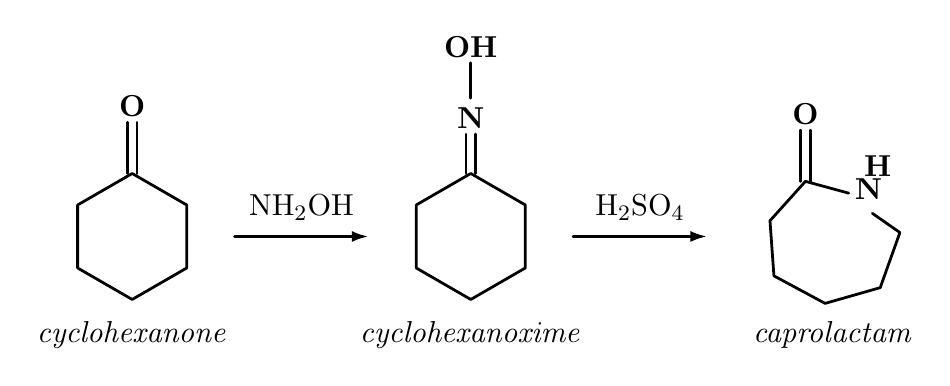
\begin{tikzpicture}[line cap=round, line join=round, font=\fontsize{11}{13}\selectfont]
    \tikzset{
        chemline/.style={line width=1.0pt},
        rxarrow/.style={line width=1.0pt, -{Latex[length=6pt, width=4pt]}}
    }

    % --- 1. Cyclohexanone ---
    \begin{scope}[shift={(0,0)}]
        % 6 cạnh: top là đỉnh (90), các đỉnh khác: 30, 330, 270, 210, 150
        \def\r{0.8}
        \coordinate (c1) at (90:\r);
        \coordinate (c2) at (30:\r);
        \coordinate (c3) at (330:\r);
        \coordinate (c4) at (270:\r);
        \coordinate (c5) at (210:\r);
        \coordinate (c6) at (150:\r);
        
        \draw[chemline] (c1) -- (c2) -- (c3) -- (c4) -- (c5) -- (c6) -- cycle;
        % Liên kết đôi =O ở đỉnh c1
        \draw[chemline] ($(c1)+(-0.06,0)$) -- ($(c1)+(-0.06,0.65)$);
        \draw[chemline] ($(c1)+(0.06,0)$) -- ($(c1)+(0.06,0.65)$);
        \node at ($(c1)+(0,0.85)$) {\textbf{O}};
        \node at (0,-1.25) {\textit{cyclohexanone}};
    \end{scope}

    % --- Mũi tên 1 ---
    \draw[rxarrow] (1.3,0) -- (3.0,0) node[midway, above=2pt] {$\mathrm{NH_2OH}$};

    % --- 2. Cyclohexanoxime ---
    \begin{scope}[shift={(4.3,0)}]
        \def\r{0.8}
        \coordinate (o1) at (90:\r);
        \coordinate (o2) at (30:\r);
        \coordinate (o3) at (330:\r);
        \coordinate (o4) at (270:\r);
        \coordinate (o5) at (210:\r);
        \coordinate (o6) at (150:\r);
        
        \draw[chemline] (o1) -- (o2) -- (o3) -- (o4) -- (o5) -- (o6) -- cycle;
        % Liên kết đôi =N-OH
        \draw[chemline] ($(o1)+(-0.06,0)$) -- ($(o1)+(-0.06,0.5)$);
        \draw[chemline] ($(o1)+(0.06,0)$) -- ($(o1)+(0.06,0.5)$);
        \node (Nnode) at ($(o1)+(0,0.7)$) {\textbf{N}};
        \draw[chemline] (Nnode.north) -- ($(Nnode.north)+(0,0.45)$) node[above=-2pt] {\textbf{OH}};
        \node at (0,-1.25) {\textit{cyclohexanoxime}};
    \end{scope}

    % --- Mũi tên 2 ---
    \draw[rxarrow] (5.6,0) -- (7.3,0) node[midway, above=2pt] {$\mathrm{H_2SO_4}$};

    % --- 3. Caprolactam (vòng 7 cạnh) ---
    \begin{scope}[shift={(8.9,0)}]
        % 7 đỉnh vòng: 
        % 1: C=O (đỉnh trên trái), 2: NH (đỉnh trên phải), 3..7
        \coordinate (v1) at (-0.35, 0.7);  % C=O
        \coordinate (v2) at (0.45, 0.6);   % N
        \coordinate (v3) at (0.85, 0.05);
        \coordinate (v4) at (0.6, -0.65);
        \coordinate (v5) at (-0.1, -0.85);
        \coordinate (v6) at (-0.75, -0.5);
        \coordinate (v7) at (-0.8, 0.2);

        \draw[chemline] (v1) -- ($(v2)+(-0.25, -0.05)$);
        \node (vN) at (v2) {\textbf{N}};
        \node at ($(v2)+(0.12,0.3)$) {\textbf{H}};
        \draw[chemline] ($(vN.south)+(0.05,-0.05)$) -- (v3) -- (v4) -- (v5) -- (v6) -- (v7) -- (v1);

        % Nhóm =O ở v1
        \draw[chemline] ($(v1)+(-0.06,0)$) -- ($(v1)+(-0.06,0.65)$);
        \draw[chemline] ($(v1)+(0.06,0)$) -- ($(v1)+(0.06,0.65)$);
        \node at ($(v1)+(0,0.85)$) {\textbf{O}};
        \node at (0,-1.25) {\textit{caprolactam}};
    \end{scope}

\end{tikzpicture}
\end{document}
